\documentclass[UTF8,fontset=fandol,11pt,a4paper]{ctexart}
\usepackage[margin=22mm]{geometry}
\usepackage{booktabs,longtable,array,graphicx,xcolor,hyperref,amsmath,needspace}
\definecolor{navy}{HTML}{20364C}\definecolor{teal}{HTML}{147D92}
\hypersetup{colorlinks=true,linkcolor=teal,urlcolor=teal}
\setlength{\parskip}{5pt}\setlength{\parindent}{0pt}
\emergencystretch=3em
\title{\color{navy}PyTorch/CUDA 可达域工程\\阶段进展与实验对照}
\author{项目阶段整理}\date{2026年9月23日}
\begin{document}\pagestyle{plain}\begin{titlepage}\maketitle\thispagestyle{empty}
\begin{center}面向首次接触项目的读者；资料整理与分支推送后暂停\end{center}
\end{titlepage}
{\setlength{\parskip}{0pt}\tableofcontents}\clearpage

\Needspace{6\baselineskip}\section*{1. 当前结论}
\addcontentsline{toc}{section}{1. 当前结论}
目标是把验证连续系统的完整可达域计算迁移到 PyTorch/\allowbreak{}CUDA，既减少耗时，又保持范围紧度及数值误差覆盖。当前已经实现可运行的完整 GPU 引擎、同任务多方对照和全轨迹范围重算；总目标尚未完成。本次按用户要求整理后暂停，不继续启动优化实验。

\small
\par\noindent
{\setlength{\tabcolsep}{2pt}\renewcommand{\arraystretch}{1.25}
\begin{tabular}{>{\raggedright\arraybackslash}p{0.175\linewidth}>{\raggedright\arraybackslash}p{0.368\linewidth}>{\raggedright\arraybackslash}p{0.377\linewidth}}
\toprule
\textbf{问题} & \textbf{已有结果} & \textbf{仍需解决} \\
\midrule
固定多项式任务是否更快 & 四项任务核心时间均优于 Huan/\allowbreak{}Xiangru strict；三项相对 Flow* 达到 $\leq$1.20 倍目标 & 原式 VDP B1 仍为 Flow* 的约 2.015 倍 \\
范围是否接近 Flow* & Brusselator 和 B32 短轨迹接近；原式 VDP 已明显优于作者 strict & VDP B1 p95/\allowbreak{}max=1.123238/\allowbreak{}1.271071，略超 1.10/\allowbreak{}1.25 \\
作者闭环控制实验是否复现 & TORA、单摆完成六组相同配置实验；CartPole 六组完整尝试 & TORA v2 全成功但偏宽；CartPole 六组都未完成全程 \\
是否有实际加速 & TORA 完整进程相对 Flow* 配对速度比约 1.802；完整范围输出减少 15.3\%–43.6\% & 单摆完整进程比 Flow* 慢约 5.5\%；输出仍有明显差距 \\
能否宣称完整严格验证器 & 已保留 plant 的严格误差路径、SR 和拒绝回滚检查 & 控制器舍入误差资格、候选统一入口与整体验收未完成 \\
\bottomrule
\end{tabular}
}
\par

\normalsize
最重要的区别：跑完不等于验证为安全，宽度接近不等于证明正确，核心求解快不等于包含启动和输出的全过程快。后文给出具体数字和相应计量边界。

\Needspace{6\baselineskip}\section*{2. 项目在解决什么问题}
\addcontentsline{toc}{section}{2. 项目在解决什么问题}
给定微分方程、一个初始状态盒和时间范围，程序要包住从盒内任意状态出发的所有可能轨迹，而非只模拟一条轨迹。状态范围越宽，下游安全判断就越容易变成 Unknown；因此速度与范围质量必须同时衡量。

Taylor model（泰勒模型）把状态表示为多项式加区间余项。多项式保留变量之间的依赖，余项承担截断及浮点误差。程序逐步组合、积分并验证候选包络；成功才提交新状态。SR（symbolic remainder，符号余项）保留跨步误差关系，减轻反复装箱造成的范围膨胀；历史队列满时按原规则重置。

原路线中，GPU 局部算子很快，但大量 CPU 组织、传输和逐小算子调度仍限制完整任务。本阶段改为沿完整 GPU 状态连续推进，并优化调度和范围观察。这里的 PyTorch 加速包含必要的定向舍入 CUDA 扩展，不是禁止一切扩展的“纯 PyTorch”改写。

\small
\par\noindent
{\setlength{\tabcolsep}{2pt}\renewcommand{\arraystretch}{1.25}
\begin{tabular}{>{\raggedright\arraybackslash}p{0.184\linewidth}>{\raggedright\arraybackslash}p{0.359\linewidth}>{\raggedright\arraybackslash}p{0.377\linewidth}}
\toprule
\textbf{模块} & \textbf{主要工作} & \textbf{如何体现进展} \\
\midrule
完整推进引擎 & 稀疏多项式、Horner 组合、CUDA 图、验证和 SR 状态处理 & 以完整1000步及真实32分区任务衡量，不用局部算子倍率代替 \\
范围输出 & 从完整 Taylor model 重建物理范围；定向舍入；原生 CPU 多项式乘法 & 输出工作量相同的五次配对，完整模型保持一致 \\
闭环 NNCS & CROWN 控制器每个周期提供控制边界，再推进连续 plant & 复用相同作者配置与模型，核对完成状态和全轨迹宽度 \\
复现与证据 & 固定版本、配置、实际库、完整日志、失败行与审计 & 同机同任务比较，并保存可重算的CSV/\allowbreak{}JSON \\
\bottomrule
\end{tabular}
}
\par

\normalsize
\Needspace{6\baselineskip}\section*{3. 三个仓库、四类实现}
\addcontentsline{toc}{section}{3. 三个仓库、四类实现}
主仓库 https:/\allowbreak{}/\allowbreak{}github.com/\allowbreak{}lsnnnnnnnn/\allowbreak{}torch\_\allowbreak{}tm\_\allowbreak{}flowpipe 负责已有工程、适配入口与实验。Huan 仓库 https:/\allowbreak{}/\allowbreak{}github.com/\allowbreak{}huanzhang12/\allowbreak{}flowstar-gpu 提供被复用和对照的 GPU 引擎。Xiangru 仓库 https:/\allowbreak{}/\allowbreak{}github.com/\allowbreak{}xiangruzh/\allowbreak{}CROWN-Reach\_\allowbreak{}Development 提供 NNCS 集成、控制器及作者 benchmark。Native Flow* 是 C++ 可达域对照，不是第四个要重写的项目，也不是无条件数学真值。

\small
\par\noindent
{\setlength{\tabcolsep}{2pt}\renewcommand{\arraystretch}{1.25}
\begin{tabular}{>{\raggedright\arraybackslash}p{0.248\linewidth}>{\raggedright\arraybackslash}p{0.322\linewidth}>{\raggedright\arraybackslash}p{0.350\linewidth}}
\toprule
\textbf{材料中的名称} & \textbf{固定版本} & \textbf{用途} \\
\midrule
我们 plant 正式比较版 & engine f53696c8；adapter 4beba860 & 四方固定原式多项式对照 \\
我们 NNCS 线性路径 v2 & engine fff9d0f5 & TORA/\allowbreak{}单摆/\allowbreak{}CartPole 新候选；尚未统一推广 \\
GPU 乘法候选 & engine d8bdc4d2 & 独立性能候选，与 fff9 分属不同实验线 \\
范围输出候选 & observer 1bc9b40f & CPU 原生乘法后端；输出语义不变 \\
Huan 原版 & d5f0b68f & 保持源码原样；strict 和 parity 分开 \\
Xiangru 原版 & 1c16d4ef，2026\_\allowbreak{}experiment & 保持源码原样；共享作者 NNCS 驱动 \\
匹配 Flow* & 722a5611 /\allowbreak{} 已冻结匹配构建 & 固定 plant 与匹配 NNCS 对照；早期 registry 使用另一历史构建，单列 \\
\bottomrule
\end{tabular}
}
\par

\normalsize
“我们”不是从零独立发明的全新算法：它建立在已有工程、Huan 引擎和保存的严格修复之上。本报告比较的是具体版本的完整实现。Huan/\allowbreak{}Xiangru 的 strict 标签与修复版 strict 的误差覆盖范围不完全相同；parity 是作者的另一数值模式，仅作复现参考。

NNCS 表中的 Huan 与 Xiangru 分别表示各自原引擎接入同一个 Xiangru 控制器驱动，不是两套独立 NNCS 产品。所有模型和驱动版本均固定；不声称这是各仓库当前最新提交的性能。

\Needspace{6\baselineskip}\section*{4. 实验口径：哪些数可以直接比较}
\addcontentsline{toc}{section}{4. 实验口径：哪些数可以直接比较}
\small
\par\noindent
{\setlength{\tabcolsep}{2pt}\renewcommand{\arraystretch}{1.25}
\begin{tabular}{>{\raggedright\arraybackslash}p{0.202\linewidth}>{\raggedright\arraybackslash}p{0.350\linewidth}>{\raggedright\arraybackslash}p{0.368\linewidth}}
\toprule
\textbf{指标} & \textbf{定义与方向} & \textbf{边界} \\
\midrule
核心求解时间 & 完整求解秒数，越小越快 & plant 包含初始化/\allowbreak{}图捕获/\allowbreak{}推进/\allowbreak{}SR/\allowbreak{}同步；排除进程启动、扩展预载、记录和范围观察 \\
完整进程时间 & 启动 runner 到退出，越小越快 & 包含 Python/\allowbreak{}库/\allowbreak{}控制器启动和最终判定；time-only 实验关闭轨迹记录；不含独立 outward 导出 \\
独立完整输出时间 & 展开多项式、求范围、gzip模型及CSV写出 & 不含求解；不能与另一场实验中位数相加冒充实测全过程 \\
宽度比 & (上界−下界) /\allowbreak{} 对应 Flow* 宽度 & 1 表示相同；大于1更宽；需同时看成功范围与绝对边界差 \\
p95 /\allowbreak{} max & 先逐通道计算，再报告最差通道 & plant 通道为 endpoint-x/\allowbreak{}y 与 tube-x/\allowbreak{}y；全部有效步/\allowbreak{}分区参与，无删最差步 \\
完成率 & 接受的分区步 /\allowbreak{} 请求分区步 & B12×200 表示2400分区步；部分失败的耗时不作为成功加速分母 \\
\bottomrule
\end{tabular}
}
\par

\normalsize
Endpoint 是每一步末端的范围；tube 是该步整个局部时间区间的范围。两者分别给出，不能用较紧的 endpoint 冒充整段包络。当前固定 plant 对照使用完整匹配的1000/\allowbreak{}20步和各步 [0,h]，不沿用早期 native 最后一步截短的观察域。

固定四方 plant 实验：4任务×6实现/\allowbreak{}模式×5次，共120个有效 time-only 样本。完整宽度另来自20条 GPU 记录任务，统一观察后65,600行/\allowbreak{}80通道本地复核。NNCS 正式计时：2任务×6组×(1次排除预跑+5次计入)，共72次调用，60次计入。CartPole 只有六组单次带记录尝试，不能称五次正式计时。

硬件为同一 huan-c4140-server-3，Intel Xeon Gold 6138、Tesla V100-SXM2 16GB；固定 plant 和 NNCS 主比较均使用单 CPU 核6、PyTorch/\allowbreak{}OMP/\allowbreak{}MKL/\allowbreak{}OpenBLAS单线程。PyTorch 2.5.1+cu121，扩展构建工具链 GCC13/\allowbreak{}CUDA12.6，实际加载库按SHA锁定。固定四方计时GPU2，后续NNCS及GPU乘法候选GPU3；输出CPU五配对固定核10。扩展缓存已经存在，不宣称首次编译冷启动。

\Needspace{6\baselineskip}\section*{5. 固定多项式：详细配置}
\addcontentsline{toc}{section}{5. 固定多项式：详细配置}
\small
\par\noindent
{\setlength{\tabcolsep}{2pt}\renewcommand{\arraystretch}{1.25}
\begin{tabular}{>{\raggedright\arraybackslash}p{0.239\linewidth}>{\raggedright\arraybackslash}p{0.340\linewidth}>{\raggedright\arraybackslash}p{0.340\linewidth}}
\toprule
\textbf{参数} & \textbf{Van der Pol} & \textbf{Brusselator} \\
\midrule
方程 & x'=y；y'=y−x−x²y & x'=1−4x+x²y；y'=3x−x²y \\
初始原盒 & x$\in$[1.1,1.4]；y$\in$[2.35,2.45] & x$\in$[1.48,1.52]；y$\in$[2.98,3.02] \\
阶数 /\allowbreak{} 固定步长 & 4 /\allowbreak{} 0.01 & 6 /\allowbreak{} 0.02 \\
B1完整任务 & 1000步，T=10 & 1000步，T=20 \\
B32吞吐任务 & 8×4真实分区，每盒20步，T=0.2 & 8×4真实分区，每盒20步，T=0.4 \\
cutoff /\allowbreak{} 余项半径 & 1e−10 /\allowbreak{} 1e−4 & 1e−10 /\allowbreak{} 1e−4 \\
SR队列容量 & 100 & 1000 \\
验证迭代上限 /\allowbreak{} stop ratio & 491 /\allowbreak{} 0.99 & 491 /\allowbreak{} 0.99 \\
\bottomrule
\end{tabular}
}
\par

\normalsize
初盒由精确十进制目标向外转成 binary64 端点；每个真实分区和实际十六进制编码均在 configs/\allowbreak{}plant\_\allowbreak{}contracts.json。B32 不是复制同一个盒32次。我们使用 Horner/\allowbreak{}graph/\allowbreak{}structural/\allowbreak{}defer\_\allowbreak{}polynomial；Huan/\allowbreak{}Xiangru 保留原版 monomial/\allowbreak{}eager 路径。相同物理任务及参数不意味着内部计算算法完全相同。

原式 VDP 的字符串固定为 y−x−x*x*y。部署试验曾用代数等价的 (1−x*x)*y−x；有限精度和区间计算的操作顺序不同，其宽度不能替代原式验收。本报告主比较全部使用原式。

\Needspace{6\baselineskip}\section*{6. 固定多项式：时间比较}
\addcontentsline{toc}{section}{6. 固定多项式：时间比较}
\small
\par\noindent
{\setlength{\tabcolsep}{2pt}\renewcommand{\arraystretch}{1.25}
\begin{tabular}{>{\raggedright\arraybackslash}p{0.230\linewidth}>{\raggedright\arraybackslash}p{0.173\linewidth}>{\raggedright\arraybackslash}p{0.173\linewidth}>{\raggedright\arraybackslash}p{0.173\linewidth}>{\raggedright\arraybackslash}p{0.173\linewidth}}
\toprule
\textbf{任务} & \textbf{我们 strict} & \textbf{Huan strict} & \textbf{Xiangru strict} & \textbf{Flow*} \\
\midrule
Van der Pol B1 & 2.921487 & 12.552073 & 12.602979 & 1.447977 \\
Van der Pol B32 & 0.769654 & 0.840225 & 0.837461 & 0.682880 \\
Brusselator B1 & 4.456490 & 16.867330 & 16.737087 & 13.847315 \\
Brusselator B32 & 0.897973 & 0.929344 & 0.935446 & 8.053289 \\
\bottomrule
\end{tabular}
}
\par

\normalsize
核心求解时间，单位秒，五次中位数。来源 S1。完整逐次数据位于 evidence/\allowbreak{}plant\_\allowbreak{}raw\_\allowbreak{}timing.json；本报告构建时重新计算了所有24组中位数。

\begin{center}\begin{minipage}{\linewidth}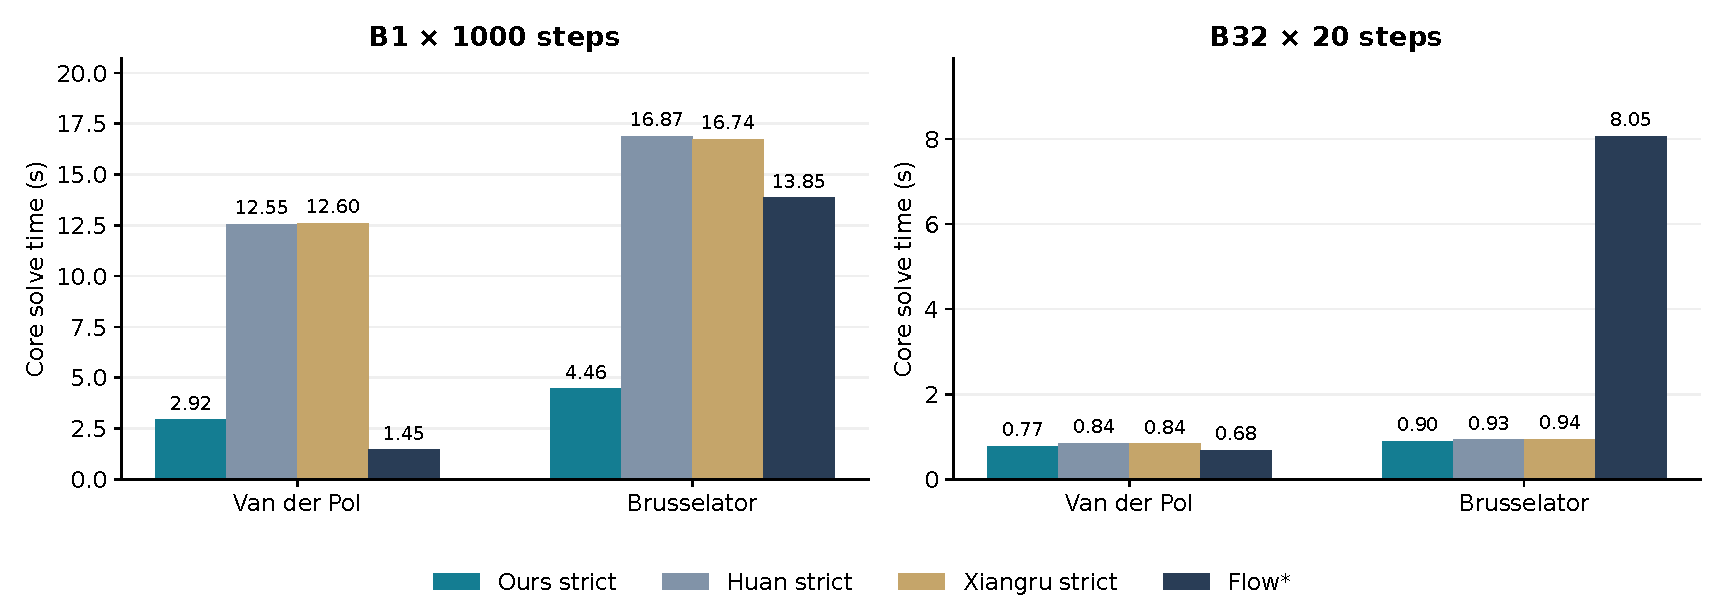
\includegraphics[width=\linewidth]{figures/plant_core.pdf}\par\small 图1：四项固定任务的完整核心求解；柱顶为秒数，各子图采用不同纵轴范围。\end{minipage}\end{center}
\small
\par\noindent
{\setlength{\tabcolsep}{2pt}\renewcommand{\arraystretch}{1.25}
\begin{tabular}{>{\raggedright\arraybackslash}p{0.322\linewidth}>{\raggedright\arraybackslash}p{0.368\linewidth}>{\raggedright\arraybackslash}p{0.230\linewidth}}
\toprule
\textbf{任务} & \textbf{我们 /\allowbreak{} Flow* 配对比中位} & \textbf{$\leq$1.20时间门槛} \\
\midrule
Van der Pol B1 & 2.015041 & 未达到 \\
Van der Pol B32 & 1.128784 & 达到 \\
Brusselator B1 & 0.321831 & 达到 \\
Brusselator B32 & 0.111111 & 达到 \\
\bottomrule
\end{tabular}
}
\par

\normalsize
Brusselator B1 和 B32 对 Flow* 有明显核心优势；VDP B32 已接近 Flow*；VDP B1 仍约慢一倍。相对 Huan/\allowbreak{}Xiangru 的 B1 加速是真实完整实现差异，但不能全部归因于“GPU”：三个被比较的引擎本来都使用 GPU，我们同时改变了表达式组织和执行调度。

\Needspace{12\baselineskip}\subsection*{把启动也算进去}
\small
\par\noindent
{\setlength{\tabcolsep}{2pt}\renewcommand{\arraystretch}{1.25}
\begin{tabular}{>{\raggedright\arraybackslash}p{0.230\linewidth}>{\raggedright\arraybackslash}p{0.173\linewidth}>{\raggedright\arraybackslash}p{0.173\linewidth}>{\raggedright\arraybackslash}p{0.173\linewidth}>{\raggedright\arraybackslash}p{0.173\linewidth}}
\toprule
\textbf{任务} & \textbf{我们 strict} & \textbf{Huan strict} & \textbf{Xiangru strict} & \textbf{Flow*} \\
\midrule
Van der Pol B1 & 5.712499 & 15.224908 & 15.224986 & 1.506329 \\
Van der Pol B32 & 3.508733 & 3.408976 & 3.508918 & 0.705000 \\
Brusselator B1 & 7.414298 & 19.630325 & 19.431740 & 13.921361 \\
Brusselator B32 & 3.709420 & 3.509076 & 3.609409 & 8.115559 \\
\bottomrule
\end{tabular}
}
\par

\normalsize
Time-only 完整进程中位秒。短 B32 任务受 Python/\allowbreak{}库启动影响很大，核心略快不保证进程更快。该列仍不包含独立范围输出。

\Needspace{6\baselineskip}\section*{7. 固定多项式：全轨迹宽度比较}
\addcontentsline{toc}{section}{7. 固定多项式：全轨迹宽度比较}
\small
\par\noindent
{\setlength{\tabcolsep}{2pt}\renewcommand{\arraystretch}{1.25}
\begin{tabular}{>{\raggedright\arraybackslash}p{0.230\linewidth}>{\raggedright\arraybackslash}p{0.230\linewidth}>{\raggedright\arraybackslash}p{0.230\linewidth}>{\raggedright\arraybackslash}p{0.230\linewidth}}
\toprule
\textbf{任务} & \textbf{我们 strict} & \textbf{Huan strict} & \textbf{Xiangru strict} \\
\midrule
Van der Pol B1 & 1.123238 /\allowbreak{} 1.271071 & 1.297229 /\allowbreak{} 1.718783 & 1.297229 /\allowbreak{} 1.718783 \\
Van der Pol B32 & 1.000597 /\allowbreak{} 1.000656 & 1.000040 /\allowbreak{} 1.000047 & 1.000040 /\allowbreak{} 1.000047 \\
Brusselator B1 & 1.012228 /\allowbreak{} 1.038326 & 1.641986 /\allowbreak{} 4.291133 & 1.641986 /\allowbreak{} 4.291133 \\
Brusselator B32 & 1.000400 /\allowbreak{} 1.000442 & 1.000007 /\allowbreak{} 1.000010 & 1.000007 /\allowbreak{} 1.000010 \\
\bottomrule
\end{tabular}
}
\par

\normalsize
每格为最差通道 p95 /\allowbreak{} max，分母是匹配 Flow*，Flow* 自身为1/\allowbreak{}1。来源 S2，全部范围按同一 outward 观察器计算；完整80通道数据及绝对边界差见附录。

我们原式 VDP B1 的 p95=1.123238、max=1.271071，仍略超过1.10/\allowbreak{}1.25；对应最差最大值出现在 endpoint-y 第982步。其余三个固定任务的最差通道均达到宽度门槛。Huan/\allowbreak{}Xiangru 在短 B32 上略紧，但长期 B1 尤其 Brusselator 的范围明显更宽。

\begin{center}\begin{minipage}{\linewidth}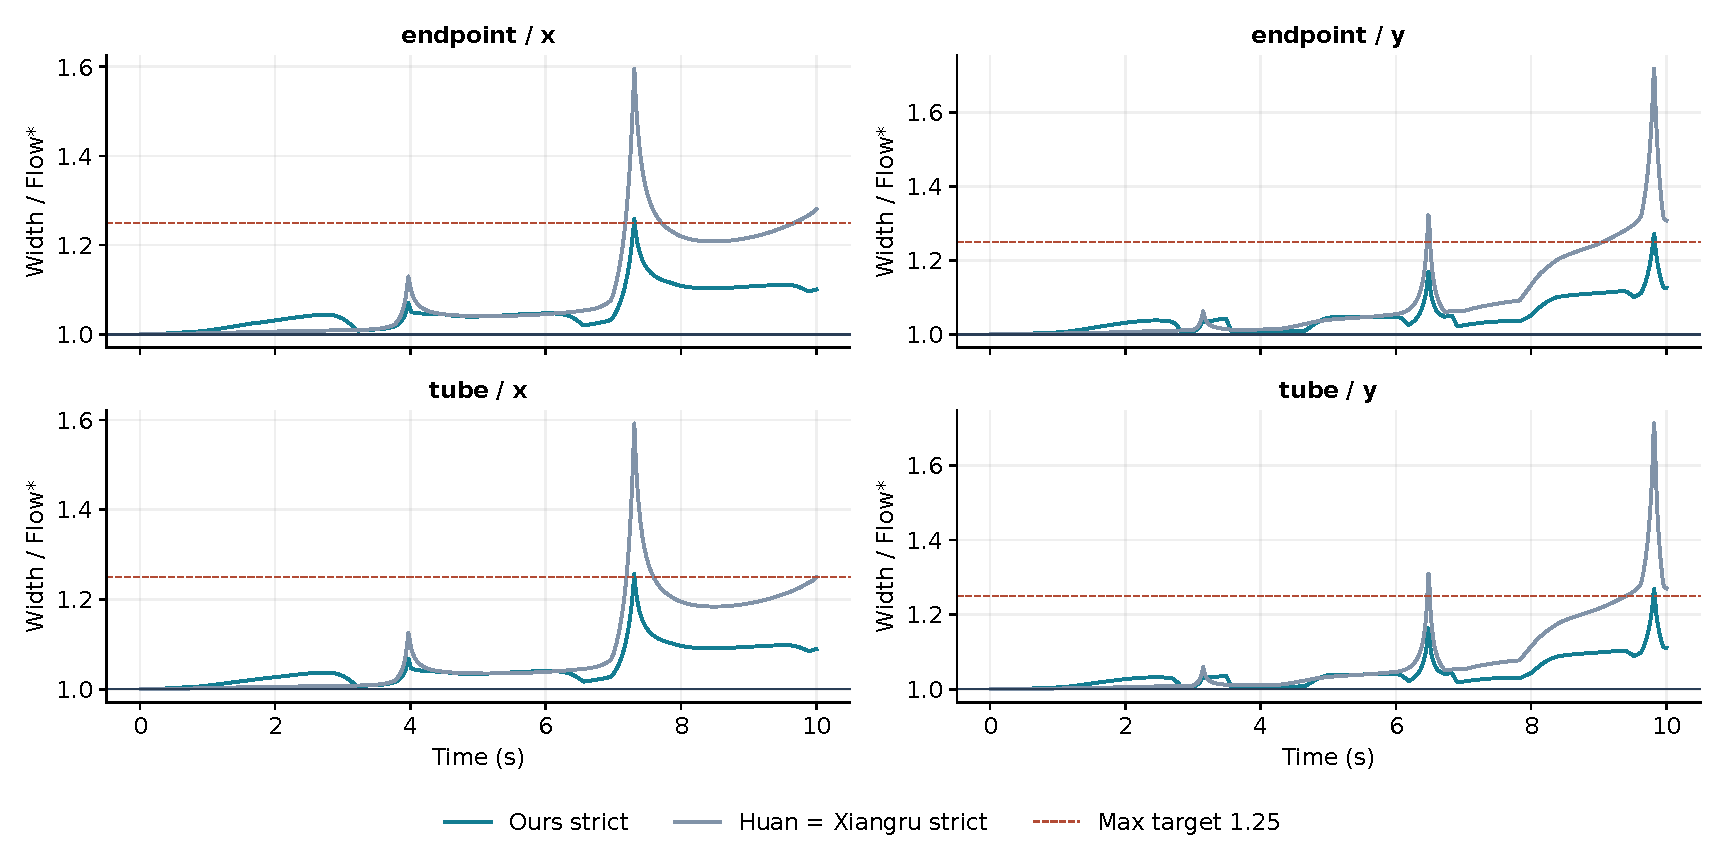
\includegraphics[width=\linewidth]{figures/van_der_pol_widths.pdf}\par\small 图2：原式 Van der Pol B1 全1000步，endpoint/\allowbreak{}tube及两个坐标分别显示。Huan与Xiangru strict曲线逐行一致后合并。\end{minipage}\end{center}
\begin{center}\begin{minipage}{\linewidth}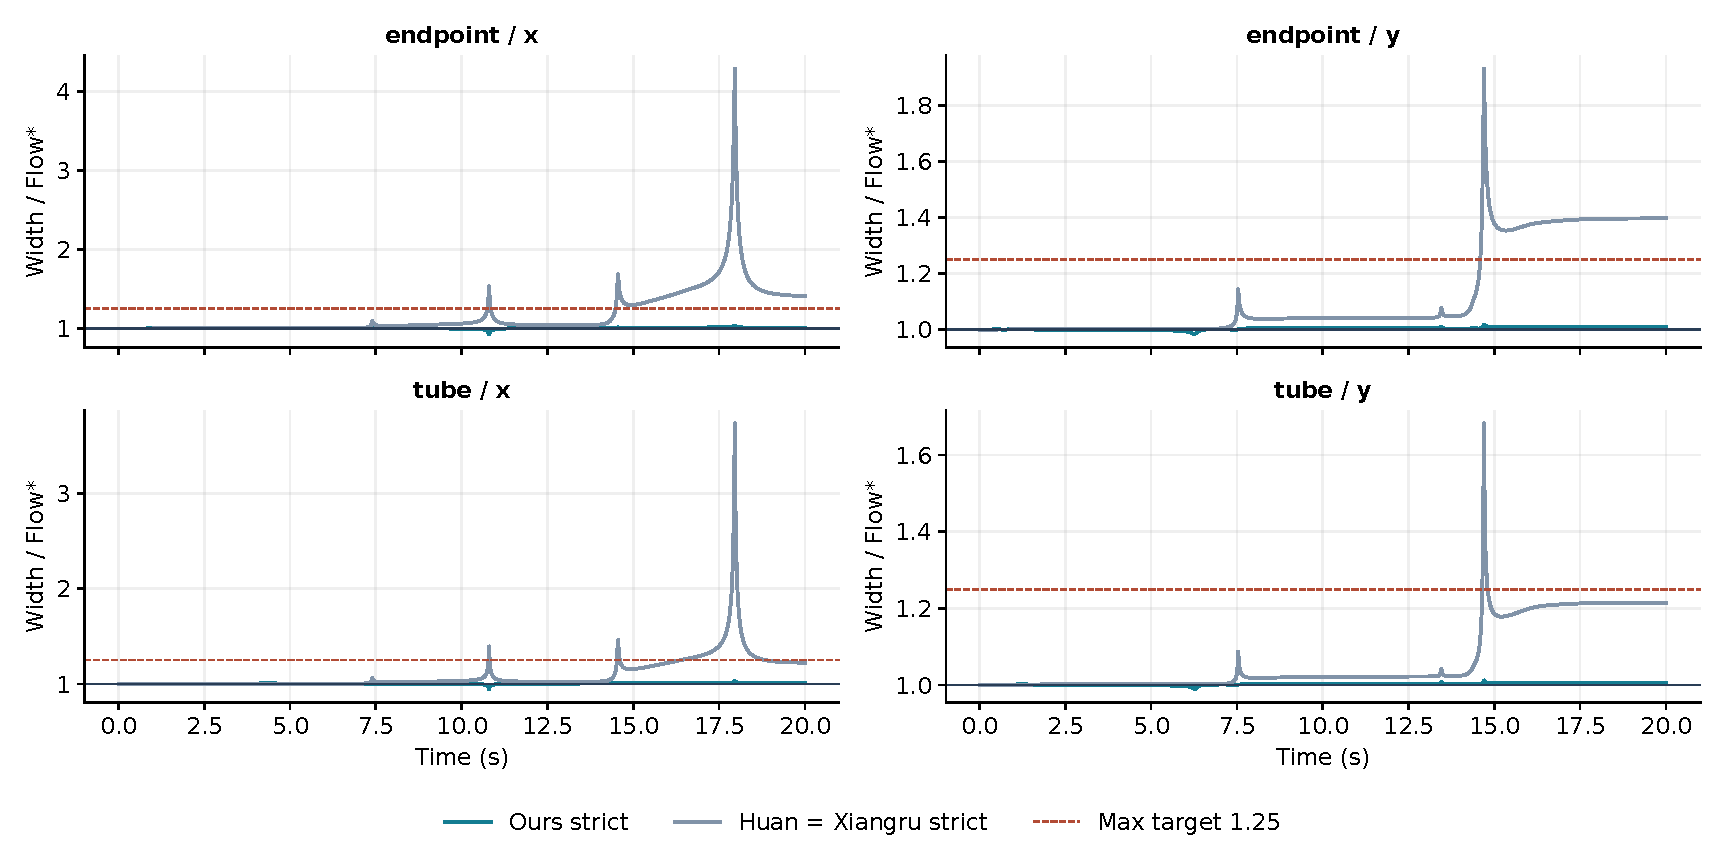
\includegraphics[width=\linewidth]{figures/brusselator_widths.pdf}\par\small 图3：Brusselator B1 全1000步。宽度优势必须与误差覆盖依据一起解读，不能独立当作正确性证明。\end{minipage}\end{center}
\Needspace{6\baselineskip}\section*{8. 作者 NNCS：配置与控制器}
\addcontentsline{toc}{section}{8. 作者 NNCS：配置与控制器}
NNCS 是神经网络控制的连续系统。每个控制周期先对当前状态集合计算神经网络控制界，再在固定控制条件下推进若干 ODE 小步；然后重复。这里对齐的不只是动力学，还包括初盒分区、周期、控制器文件、输入布局、传输精度和判定时域。

\small
\par\noindent
{\setlength{\tabcolsep}{2pt}\renewcommand{\arraystretch}{1.25}
\begin{tabular}{>{\raggedright\arraybackslash}p{0.258\linewidth}>{\raggedright\arraybackslash}p{0.221\linewidth}>{\raggedright\arraybackslash}p{0.221\linewidth}>{\raggedright\arraybackslash}p{0.221\linewidth}}
\toprule
\textbf{参数} & \textbf{TORA} & \textbf{Single Pendulum} & \textbf{CartPole} \\
\midrule
物理维度 /\allowbreak{} 总状态 & 4 /\allowbreak{} 6（含t,u） & 2 /\allowbreak{} 4（含t,u） & 4 /\allowbreak{} 6（含t,u） \\
B /\allowbreak{} 每盒ODE步数 & 12 /\allowbreak{} 200 & 1 /\allowbreak{} 100 & 1 /\allowbreak{} 200 \\
阶数 /\allowbreak{} ODE步长 & 3 /\allowbreak{} 0.1 & 2 /\allowbreak{} 0.01 & 6 /\allowbreak{} 0.005 \\
控制周期 /\allowbreak{} 周期数 & 1.0 /\allowbreak{} 20 & 0.05 /\allowbreak{} 20 & 0.02 /\allowbreak{} 50 \\
总时长 & 20 & 1 & 1 \\
cutoff & 1e−6 & 1e−6 & 1e−6 \\
余项猜测区间 & [−0.01,0.01] & [−0.01,0.01] & [−0.1,0.1] \\
空间分区 & x1分4份、x2分3份 & 不分区 & 没有split\_\allowbreak{}vars，实际B1 \\
SR实际队列容量 & 1000（驱动固定值） & 1000（驱动固定值） & 1000（驱动固定值） \\
输入shape & [-1,1,1,4] & [-1,1,2] & [-1,4] \\
\bottomrule
\end{tabular}
}
\par

\normalsize
三个共同实验均用相同 ONNX 模型、box CROWN、same-slope relaxation、flat 输入映射和 rpc-float32 传输合同；输出 scale=1、offset=0。GPU 使用共享 Xiangru 驱动，保留我们修复后的 endpoint 算术；native 使用既有 RPC 服务与固定步数/\allowbreak{}共同 binary64 初盒支路。原 native 每周期尾步浮点截短的原始支路单独保留，不与固定步数支路混用。

\small
\par\noindent
{\setlength{\tabcolsep}{2pt}\renewcommand{\arraystretch}{1.25}
\begin{tabular}{>{\raggedright\arraybackslash}p{0.138\linewidth}>{\raggedright\arraybackslash}p{0.359\linewidth}>{\raggedright\arraybackslash}p{0.423\linewidth}}
\toprule
\textbf{任务} & \textbf{初始物理状态} & \textbf{动力学} \\
\midrule
TORA & x1=[0.6,0.7]；x2=[−0.7,−0.6]；x3=[−0.4,−0.3]；x4=[0.5,0.6] & x1'=x2；x2'=−x1+0.1sin(x3)；x3'=x4；x4'=u−10 \\
单摆 & x1=[1,1.175]；x2=[0,0.2] & x1'=x2；x2'=2sin(x1)+8u \\
CartPole & x1=[−0.0375,−0.03125]；x2=[−0.015625,−0.0125]；x3=[−0.00625,0]；x4=[−0.007375,−0.00625] & x1'=x2；x2'=2u；x3'=x4；x4'=(0.08·0.41·(9.8sin(x3)−2u cos(x3))−0.0021x4)/\allowbreak{}0.0105 \\
\bottomrule
\end{tabular}
}
\par

\normalsize
所有 NNCS 的附加状态 t、u 初值为0；周期内 t$\prime$=1、u$\prime$=0。原始 YAML 与精确执行版本 *\_\allowbreak{}executed.yaml 同时保留。完整 YAML 保留安全/\allowbreak{}不安全/\allowbreak{}目标约束、模型路径及形状等字段。TORA 使用 controllerTora.onnx；单摆使用 controller\_\allowbreak{}single\_\allowbreak{}pendulum.onnx；CartPole 使用 model.onnx。SHA 身份记录随 evidence/\allowbreak{} 中的 *\_\allowbreak{}identity.json、campaign 与 contract 交付，权重文件本身保留服务器。

CartPole 选的是作者 registry 的历史小初盒 full profile。它与4096分区 profile、大初盒10秒 ARCH-COMP profile不同。原 src/\allowbreak{}configs/\allowbreak{}cartpole.yaml 的 ODE步长0.05大于控制周期0.02，是另一份无效配置，没有据此猜测修参数。本次有效配置为 registry 原值，实际运行与本报告一致。

\Needspace{6\baselineskip}\section*{9. TORA 与单摆：相同实验的时间和宽度}
\addcontentsline{toc}{section}{9. TORA 与单摆：相同实验的时间和宽度}
\Needspace{12\baselineskip}\subsection*{TORA：B12×200}
\small
\par\noindent
{\setlength{\tabcolsep}{2pt}\renewcommand{\arraystretch}{1.25}
\begin{tabular}{>{\raggedright\arraybackslash}p{0.202\linewidth}>{\raggedright\arraybackslash}p{0.147\linewidth}>{\raggedright\arraybackslash}p{0.175\linewidth}>{\raggedright\arraybackslash}p{0.147\linewidth}>{\raggedright\arraybackslash}p{0.248\linewidth}}
\toprule
\textbf{实现} & \textbf{进程中位秒} & \textbf{五次最小–最大} & \textbf{成功分区步} & \textbf{全程p95 /\allowbreak{} max} \\
\midrule
我们 strict v2 & 6.765149 & 6.716–6.893 & 2400/\allowbreak{}2400 & 1.592229 /\allowbreak{} 2.710606 \\
Huan strict & 7.767449 & 7.712–7.830 & 2357/\allowbreak{}2400 & 未完整 \\
Xiangru strict & 7.703708 & 7.666–7.718 & 2357/\allowbreak{}2400 & 未完整 \\
Flow* & 12.237700 & 12.191–12.259 & 2400/\allowbreak{}2400 & 1.000000 /\allowbreak{} 1.000000 \\
Huan parity & 7.615457 & 7.557–7.619 & 2400/\allowbreak{}2400 & 1.000000 /\allowbreak{} 1.000000 \\
Xiangru parity & 7.663851 & 7.609–7.669 & 2400/\allowbreak{}2400 & 1.000000 /\allowbreak{} 1.000000 \\
\bottomrule
\end{tabular}
}
\par

\normalsize
\Needspace{12\baselineskip}\subsection*{Single Pendulum：B1×100}
\small
\par\noindent
{\setlength{\tabcolsep}{2pt}\renewcommand{\arraystretch}{1.25}
\begin{tabular}{>{\raggedright\arraybackslash}p{0.202\linewidth}>{\raggedright\arraybackslash}p{0.147\linewidth}>{\raggedright\arraybackslash}p{0.175\linewidth}>{\raggedright\arraybackslash}p{0.147\linewidth}>{\raggedright\arraybackslash}p{0.248\linewidth}}
\toprule
\textbf{实现} & \textbf{进程中位秒} & \textbf{五次最小–最大} & \textbf{成功分区步} & \textbf{全程p95 /\allowbreak{} max} \\
\midrule
我们 strict v2 & 5.265644 & 5.214–5.446 & 100/\allowbreak{}100 & 1.036731 /\allowbreak{} 1.040936 \\
Huan strict & 5.615390 & 5.604–5.806 & 100/\allowbreak{}100 & 1.067393 /\allowbreak{} 1.075450 \\
Xiangru strict & 5.609886 & 5.602–5.652 & 100/\allowbreak{}100 & 1.067393 /\allowbreak{} 1.075450 \\
Flow* & 4.986815 & 4.985–5.041 & 100/\allowbreak{}100 & 1.000000 /\allowbreak{} 1.000000 \\
Huan parity & 5.558743 & 5.551–5.564 & 100/\allowbreak{}100 & 1.000000 /\allowbreak{} 1.000000 \\
Xiangru parity & 5.569671 & 5.549–5.605 & 100/\allowbreak{}100 & 1.000000 /\allowbreak{} 1.000000 \\
\bottomrule
\end{tabular}
}
\par

\normalsize
来源 S3。时间为五次完整进程调用，不是作者内部打印的 plant 计时。宽度来自同配置的独立完整数值记录；无记录计时样本检查身份、完成状态及完整GPU任务最终 HULL 的12位有效数字一致，未对每次计时的全部中间状态重采样。

\begin{center}\begin{minipage}{\linewidth}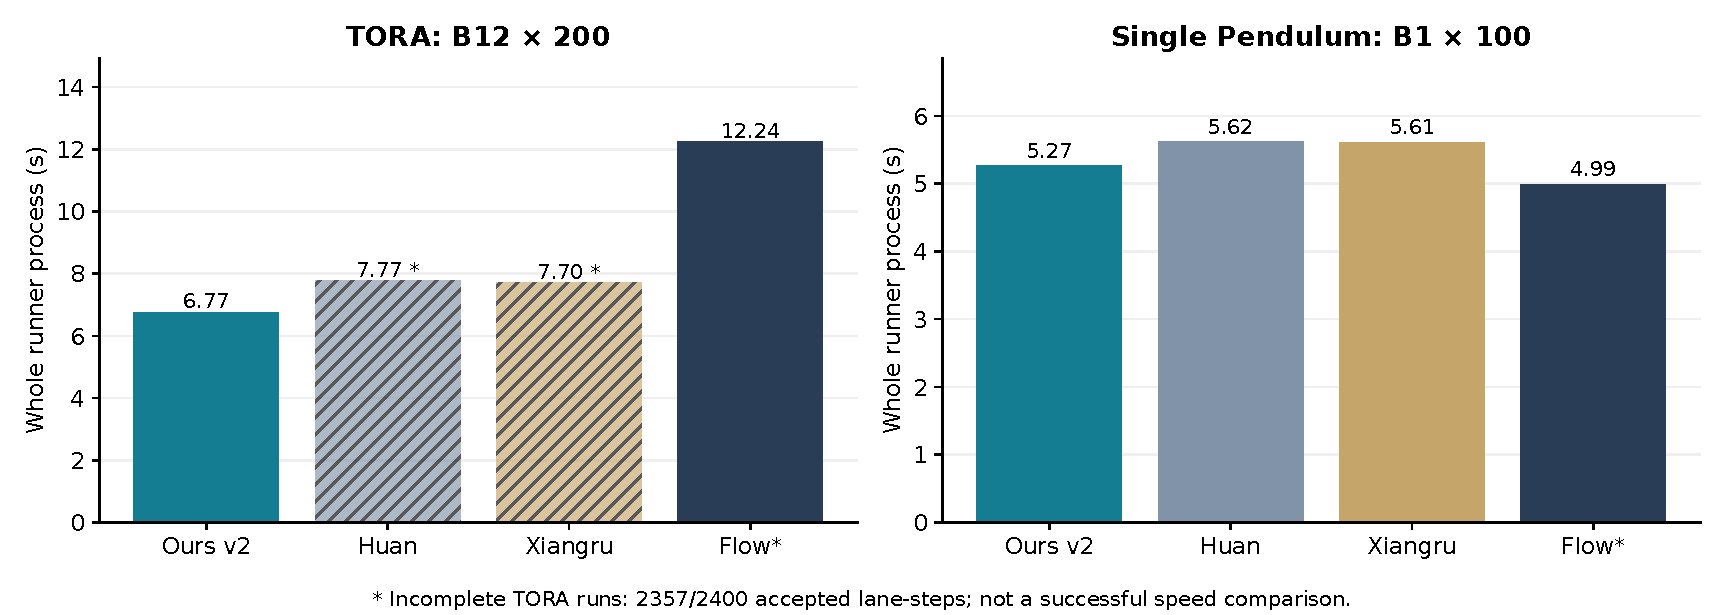
\includegraphics[width=\linewidth]{figures/nncs_time.pdf}\par\small 图4：六组计时表中的 strict 和 native 主比较。TORA 的作者 strict 未完整，斜线柱仅展示耗时，不计算成功加速比。\end{minipage}\end{center}
TORA：新 v2 全2400分区步成功，五次逐轮 native/\allowbreak{}我们 进程时间比中位为1.802031。Huan/\allowbreak{}Xiangru strict 为2357/\allowbreak{}2400，不能把其不完整时间作为成功速度基准。Parity 全程成功且范围几乎与 Flow* 一致，但不能拿它替代 strict 的保证。

单摆：所有实现都完成100步。我们宽度p95/\allowbreak{}max为1.036731/\allowbreak{}1.040936，优于原版 strict 的1.067393/\allowbreak{}1.075450。完整进程我们5.266秒、Flow*4.987秒，逐轮native/\allowbreak{}我们为0.947724，换算我们约慢5.5\%。内部计时看起来更快，正说明计时边界不能混用。

\begin{center}\begin{minipage}{\linewidth}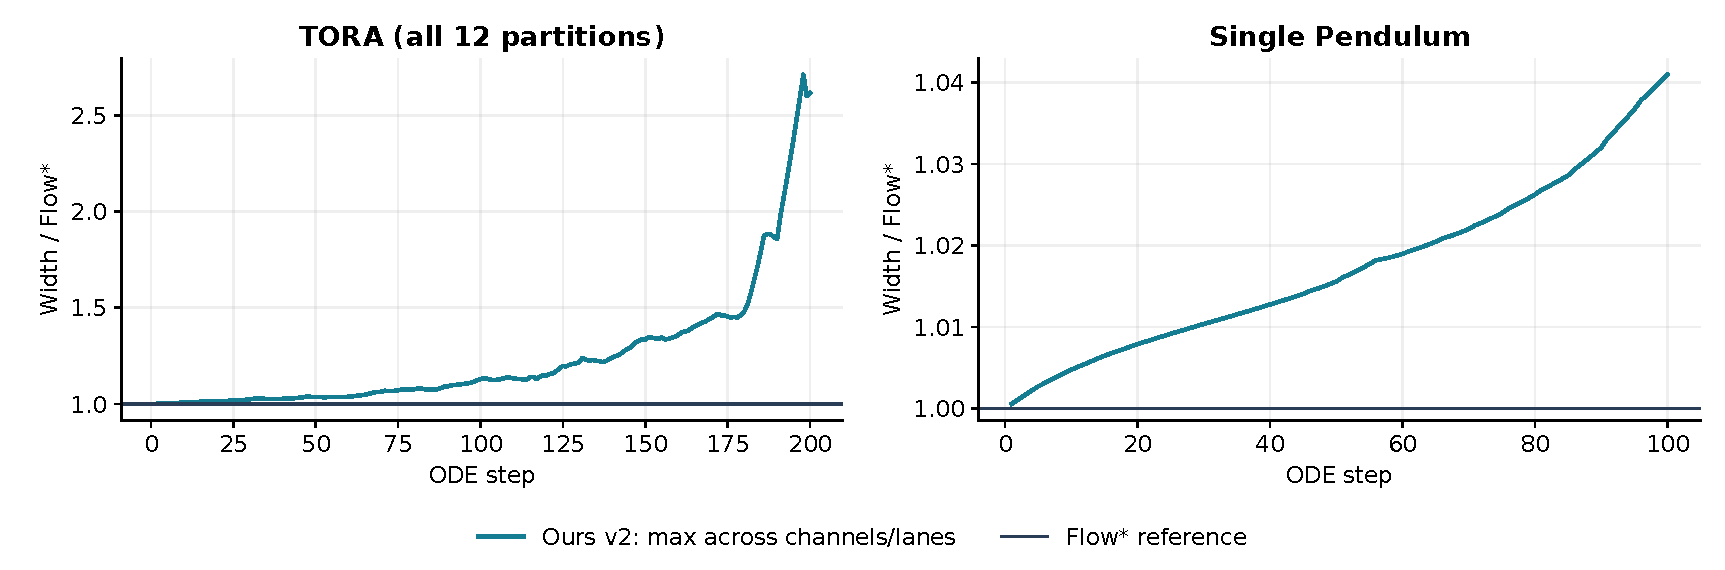
\includegraphics[width=\linewidth]{figures/nncs_width.pdf}\par\small 图5：我们 v2 全轨迹每一步的最坏通道/\allowbreak{}分区宽度比。此图的逐时刻最大曲线与“先逐通道p95再取最坏值”不同，表中的统计仍按正式定义。\end{minipage}\end{center}
\Needspace{12\baselineskip}\subsection*{主要数值改进：TORA 从部分失败到全部成功}
\small
\par\noindent
{\setlength{\tabcolsep}{2pt}\renewcommand{\arraystretch}{1.25}
\begin{tabular}{>{\raggedright\arraybackslash}p{0.230\linewidth}>{\raggedright\arraybackslash}p{0.212\linewidth}>{\raggedright\arraybackslash}p{0.478\linewidth}}
\toprule
\textbf{阶段} & \textbf{成功分区步} & \textbf{解释} \\
\midrule
初始严格版 & 2354/\allowbreak{}2400 & 首个失败出现在第189步 \\
直接变量v1 & 2393/\allowbreak{}2400 & 首个失败推迟到第197步 \\
线性路径v2 & 2400/\allowbreak{}2400 & 仅沿加/\allowbreak{}减/\allowbreak{}取负到输出的路径保留完整多项式，再由原验证积分承担误差 \\
\bottomrule
\end{tabular}
}
\par

\normalsize
与初始版本共同前188步比较，最差 p95/\allowbreak{}max 从2.555528/\allowbreak{}8.854653改善到1.383703/\allowbreak{}1.884253；不是拿旧部分轨迹分布与新完整轨迹直接比较。新v2全程仍为1.592229/\allowbreak{}2.710606，后段范围偏宽尚未解决。所有非线性消费者仍阻止这一线性保留策略，未通过全局清零余项取得表面紧度。

\Needspace{6\baselineskip}\section*{10. CartPole：六组都未完成全程}
\addcontentsline{toc}{section}{10. CartPole：六组都未完成全程}
\small
\par\noindent
{\setlength{\tabcolsep}{2pt}\renewcommand{\arraystretch}{1.25}
\begin{tabular}{>{\raggedright\arraybackslash}p{0.221\linewidth}>{\raggedright\arraybackslash}p{0.202\linewidth}>{\raggedright\arraybackslash}p{0.156\linewidth}>{\raggedright\arraybackslash}p{0.340\linewidth}}
\toprule
\textbf{实现} & \textbf{单次带记录进程秒} & \textbf{成功步} & \textbf{共同前141步p95 /\allowbreak{} max} \\
\midrule
Flow* & 8.933 & 141/\allowbreak{}200 & 1 /\allowbreak{} 1 \\
我们 strict v2 & 18.142 & 156/\allowbreak{}200 & 1.000118432 /\allowbreak{} 1.000134190 \\
Huan strict & 19.249 & 156/\allowbreak{}200 & 0.999999993 /\allowbreak{} 1.000032320 \\
Xiangru strict & 19.192 & 156/\allowbreak{}200 & 0.999999993 /\allowbreak{} 1.000032320 \\
Huan parity & 19.248 & 156/\allowbreak{}200 & 0.999999993 /\allowbreak{} 1.000032262 \\
Xiangru parity & 19.214 & 156/\allowbreak{}200 & 0.999999993 /\allowbreak{} 1.000032262 \\
\bottomrule
\end{tabular}
}
\par

\normalsize
来源 S4。Native 保存141步成功模型后提前终止；五个GPU实现均接受156步，第157步明确拒绝，随后43步未尝试。只有共同前141步能计算相对 native 的宽度比；GPU第142–156步有范围但无native分母，比例留空。

共同前缀范围非常接近，但这既不表示200步全程通过，也不能解释两类实现拒绝时刻为何不同。当前只确认输出与停止位置，尚未给出拒绝差异的完整因果分析。完成步数、记录方式和计时边界不同，不对上表计算加速比。9,600请求行、7,368可用物理范围和12项完整Fraction检查已经本地复核。

\Needspace{6\baselineskip}\section*{11. 实际加速进展与代价}
\addcontentsline{toc}{section}{11. 实际加速进展与代价}
大方向上的加速包括：让完整状态驻留GPU；减少稀疏组合的重复组织和小kernel调度；将固定流程捕获为CUDA图；复用SR准备工作；加快向外舍入的范围展开。下面两项有独立的旧/\allowbreak{}新五配对证据，不能与更早作者实验的单次时间混成新配对。

\small
\par\noindent
{\setlength{\tabcolsep}{2pt}\renewcommand{\arraystretch}{1.25}
\begin{tabular}{>{\raggedright\arraybackslash}p{0.285\linewidth}>{\raggedright\arraybackslash}p{0.212\linewidth}>{\raggedright\arraybackslash}p{0.212\linewidth}>{\raggedright\arraybackslash}p{0.212\linewidth}}
\toprule
\textbf{完整输出任务} & \textbf{旧中位秒} & \textbf{新中位秒} & \textbf{配对耗时下降} \\
\midrule
VDP B1 & 7.266908 & 5.688225 & 21.8\% \\
VDP B32 & 2.744789 & 2.324720 & 15.3\% \\
Brusselator B1 & 74.380369 & 41.760145 & 43.6\% \\
Brusselator B32 & 10.311151 & 7.933436 & 23.1\% \\
\bottomrule
\end{tabular}
}
\par

\normalsize
来源 S5，40个输出样本、20对完整模型在服务器一致，131,200行范围与冻结四方表本地对照。输出后端仍包含CPU工作：这项提升来自将多项式乘法放入原生CPU实现，保留操作/\allowbreak{}舍入顺序；不能称为纯GPU加速。Brusselator输出从约74秒降至约42秒，但原版单次约10.6秒，差距仍大。

\small
\par\noindent
{\setlength{\tabcolsep}{2pt}\renewcommand{\arraystretch}{1.25}
\begin{tabular}{>{\raggedright\arraybackslash}p{0.368\linewidth}>{\raggedright\arraybackslash}p{0.184\linewidth}>{\raggedright\arraybackslash}p{0.184\linewidth}>{\raggedright\arraybackslash}p{0.184\linewidth}}
\toprule
\textbf{GPU候选试验} & \textbf{f536旧中位秒} & \textbf{d8新中位秒} & \textbf{配对变化} \\
\midrule
VDP B1×1000，regrouped RHS & 2.831174 & 2.733734 & 下降3.30\% \\
\bottomrule
\end{tabular}
}
\par

\normalsize
该GPU试验显式使用第九个乘法误差融合库，五对逐对比中位0.966981；完整模型逐位资格保持。它没有新跑native，因此不能借用历史native时间声称新的正式Flow*比；其regrouped RHS也不能替代本报告原式主对照。

暂停前最后一次诊断已经完成：f536与d8在原式VDP上各做完整计时/\allowbreak{}trace诊断及阶段测量，六次完整1000步数值记录均与冻结原式一致。最后捕获的compose图单独重放中位约541→453微秒，kernel数288→252；normalize约238微秒，validpost约229微秒。该图测量排除了输入拷贝，也不是完整事务或五次正式任务计时，仅说明继续减少组合调度仍是可检验方向。

\Needspace{6\baselineskip}\section*{12. 更广 benchmark 覆盖到哪里}
\addcontentsline{toc}{section}{12. 更广 benchmark 覆盖到哪里}
已经盘点Huan的12个原生plant registry任务、Xiangru的14个NNCS配置及一个单列的native QUAD合同。27个合同不等于27个任务都完成四方计时和宽度；目前完整多方主比较集中在四个固定plant任务、TORA、单摆和CartPole。

12个native registry plant的原时域尝试中11个完成，Robertson在原h=0.1/\allowbreak{}order3/\allowbreak{}queue0配置第一步拒绝；早期严格CPU短前缀10/\allowbreak{}12完成，Quadrotor超时。它们是可运行性筛查，使用不同历史版本与计时边界，不并入本报告GPU速度排名。

\small
\par\noindent
{\setlength{\tabcolsep}{2pt}\renewcommand{\arraystretch}{1.25}
\begin{tabular}{>{\raggedright\arraybackslash}p{0.368\linewidth}>{\raggedright\arraybackslash}p{0.138\linewidth}>{\raggedright\arraybackslash}p{0.166\linewidth}>{\raggedright\arraybackslash}p{0.248\linewidth}}
\toprule
\textbf{早期NNCS全时域筛查} & \textbf{请求B×步} & \textbf{接受分区步} & \textbf{该次运行状态} \\
\midrule
acc & 1×50 & 50 & 完整接受 \\
single\_\allowbreak{}pendulum & 1×100 & 100 & 完整接受 \\
tora\_\allowbreak{}homogeneous & 12×200 & 2354 & 完整接受 \\
attitude\_\allowbreak{}control & 1×60 & 60 & 完整接受 \\
cartpole & 1×200 & 156 & 数值拒绝 \\
double\_\allowbreak{}pendulum\_\allowbreak{}less\_\allowbreak{}robust & 225×100 & 22500 & 完整接受 \\
double\_\allowbreak{}pendulum\_\allowbreak{}more\_\allowbreak{}robust & 1×80 & 66 & Unsafe协议提前停止 \\
tora\_\allowbreak{}relu\_\allowbreak{}tanh & 1×500 & 500 & 完整接受 \\
tora\_\allowbreak{}sigmoid & 1×500 & 500 & 完整接受 \\
unicycle & 1×500 & 500 & 完整接受 \\
nav\_\allowbreak{}robust & 25×600 & 15000 & 完整接受 \\
nav\_\allowbreak{}standard & 640×600 & 384000 & 完整接受 \\
\bottomrule
\end{tabular}
}
\par

\normalsize
这是9d83162d历史版本、native-f64控制器传输的独立筛查；12项中9项完整接受。不能与后续rpc-float32多方实验直接位比较；TORA后续v2已经补到完整成功。DP-more的66/\allowbreak{}80是Unsafe协议提前停止，不是程序属性异常。Airplane有规模/\allowbreak{}内存限制，原QUAD YAML参数无效，另立的native QUAD合同不能代替原配置。

\Needspace{6\baselineskip}\section*{13. 数值保证、尚未达标项与暂停点}
\addcontentsline{toc}{section}{13. 数值保证、尚未达标项与暂停点}
本阶段保留了strict/\allowbreak{}outward路径、完整误差余项、SR历史及原子事务：验证失败不能把未接受状态提交给下一步。采用源码身份、实际库身份、精确有理数Fraction检查、CPU/\allowbreak{}CUDA路径、跨SR重置和混合失败回滚测试共同限定可用范围。完整模型一致和范围重算是证据的一部分，不是全程序形式证明。

完整NNCS仍有明确缺口：CROWN及控制器仿射结果采用round-to-nearest计算/\allowbreak{}注入，尚未完成全过程向外舍入误差资格。因此“strict”在这些NNCS实验中首先描述plant设置；不能称已获得端到端严格控制系统证书。

\small
\par\noindent
{\setlength{\tabcolsep}{2pt}\renewcommand{\arraystretch}{1.25}
\begin{tabular}{>{\raggedright\arraybackslash}p{0.313\linewidth}>{\raggedright\arraybackslash}p{0.405\linewidth}>{\raggedright\arraybackslash}p{0.202\linewidth}}
\toprule
\textbf{总目标要求} & \textbf{当前证据} & \textbf{状态} \\
\midrule
四固定任务核心$\leq$1.20×native & VDP B1约2.015；其余三项达到 & 未全部达到 \\
每通道p95$\leq$1.10、max$\leq$1.25 & 原式VDP B1为1.123238/\allowbreak{}1.271071；其他三项达到 & 未全部达到 \\
实测改善完整范围输出 & 四任务输出五配对改善15.3\%–43.6\% & 已取得阶段证据 \\
五次匹配配对和完整宽度 & 固定plant已完成；TORA/\allowbreak{}单摆另完成；CartPole不完整 & 按任务分别成立 \\
统一入口与可复现交付 & plant基线入口已在adapter；fff9/\allowbreak{}d8/\allowbreak{}输出候选仍独立 & 候选尚未全面集成 \\
作者benchmark和严格NNCS & 已经扩展并如实保存失败；控制器资格未完成 & 未完成 \\
\bottomrule
\end{tabular}
}
\par

\normalsize
用户要求完成本次文档、幻灯片及新分支推送后暂停。暂停时不再开启新优化或benchmark。未来恢复时优先处理原式VDP核心成本与最差步宽度、TORA末段范围及控制器误差资格，再做新的五次同任务验收；这些是待执行方向，不是本次已经实现的成果。

\Needspace{6\baselineskip}\section*{附录A. endpoint/\allowbreak{}tube四通道具体宽度}
\addcontentsline{toc}{section}{附录A. endpoint/\allowbreak{}tube四通道具体宽度}
以下保留原式固定任务的全部strict通道统计。max绝对边界差是上下边界差绝对值的较大者，单位随状态坐标；零native宽度计数在原始JSON中保留。完整CSV另含所有parity数据。

\Needspace{12\baselineskip}\subsection*{Van der Pol B1}
\small
\par\noindent
{\setlength{\tabcolsep}{2pt}\renewcommand{\arraystretch}{1.25}
\begin{tabular}{>{\raggedright\arraybackslash}p{0.138\linewidth}>{\raggedright\arraybackslash}p{0.221\linewidth}>{\raggedright\arraybackslash}p{0.175\linewidth}>{\raggedright\arraybackslash}p{0.175\linewidth}>{\raggedright\arraybackslash}p{0.212\linewidth}}
\toprule
\textbf{实现} & \textbf{通道} & \textbf{p95} & \textbf{max} & \textbf{最大绝对边界差} \\
\midrule
我们 & endpoint\_\allowbreak{}x & 1.123238 & 1.258442 & 0.0114757 \\
我们 & endpoint\_\allowbreak{}y & 1.116326 & 1.271071 & 0.0174555 \\
我们 & tube\_\allowbreak{}x & 1.110254 & 1.256735 & 0.0114757 \\
我们 & tube\_\allowbreak{}y & 1.103006 & 1.268970 & 0.0174551 \\
Huan & endpoint\_\allowbreak{}x & 1.270211 & 1.596117 & 0.0287459 \\
Huan & endpoint\_\allowbreak{}y & 1.297229 & 1.718783 & 0.0426141 \\
Huan & tube\_\allowbreak{}x & 1.241658 & 1.592176 & 0.0287352 \\
Huan & tube\_\allowbreak{}y & 1.262980 & 1.713198 & 0.0423679 \\
Xiangru & endpoint\_\allowbreak{}x & 1.270211 & 1.596117 & 0.0287459 \\
Xiangru & endpoint\_\allowbreak{}y & 1.297229 & 1.718783 & 0.0426141 \\
Xiangru & tube\_\allowbreak{}x & 1.241658 & 1.592176 & 0.0287352 \\
Xiangru & tube\_\allowbreak{}y & 1.262980 & 1.713198 & 0.0423679 \\
\bottomrule
\end{tabular}
}
\par

\normalsize
\Needspace{12\baselineskip}\subsection*{Van der Pol B32}
\small
\par\noindent
{\setlength{\tabcolsep}{2pt}\renewcommand{\arraystretch}{1.25}
\begin{tabular}{>{\raggedright\arraybackslash}p{0.138\linewidth}>{\raggedright\arraybackslash}p{0.221\linewidth}>{\raggedright\arraybackslash}p{0.175\linewidth}>{\raggedright\arraybackslash}p{0.175\linewidth}>{\raggedright\arraybackslash}p{0.212\linewidth}}
\toprule
\textbf{实现} & \textbf{通道} & \textbf{p95} & \textbf{max} & \textbf{最大绝对边界差} \\
\midrule
我们 & endpoint\_\allowbreak{}x & 1.000597 & 1.000656 & 1.59622e-05 \\
我们 & endpoint\_\allowbreak{}y & 1.000016 & 1.000025 & 3.31476e-06 \\
我们 & tube\_\allowbreak{}x & 1.000408 & 1.000447 & 1.59662e-05 \\
我们 & tube\_\allowbreak{}y & 1.000010 & 1.000014 & 3.24219e-06 \\
Huan & endpoint\_\allowbreak{}x & 1.000018 & 1.000021 & 4.43563e-07 \\
Huan & endpoint\_\allowbreak{}y & 1.000040 & 1.000047 & 1.5411e-06 \\
Huan & tube\_\allowbreak{}x & 1.000012 & 1.000015 & 4.43306e-07 \\
Huan & tube\_\allowbreak{}y & 1.000022 & 1.000025 & 1.54017e-06 \\
Xiangru & endpoint\_\allowbreak{}x & 1.000018 & 1.000021 & 4.43563e-07 \\
Xiangru & endpoint\_\allowbreak{}y & 1.000040 & 1.000047 & 1.5411e-06 \\
Xiangru & tube\_\allowbreak{}x & 1.000012 & 1.000015 & 4.43306e-07 \\
Xiangru & tube\_\allowbreak{}y & 1.000022 & 1.000025 & 1.54017e-06 \\
\bottomrule
\end{tabular}
}
\par

\normalsize
\Needspace{12\baselineskip}\subsection*{Brusselator B1}
\small
\par\noindent
{\setlength{\tabcolsep}{2pt}\renewcommand{\arraystretch}{1.25}
\begin{tabular}{>{\raggedright\arraybackslash}p{0.138\linewidth}>{\raggedright\arraybackslash}p{0.221\linewidth}>{\raggedright\arraybackslash}p{0.175\linewidth}>{\raggedright\arraybackslash}p{0.175\linewidth}>{\raggedright\arraybackslash}p{0.212\linewidth}}
\toprule
\textbf{实现} & \textbf{通道} & \textbf{p95} & \textbf{max} & \textbf{最大绝对边界差} \\
\midrule
我们 & endpoint\_\allowbreak{}x & 1.012228 & 1.038326 & 0.000544567 \\
我们 & endpoint\_\allowbreak{}y & 1.009878 & 1.018139 & 0.000592378 \\
我们 & tube\_\allowbreak{}x & 1.006765 & 1.030982 & 0.00054031 \\
我们 & tube\_\allowbreak{}y & 1.005331 & 1.011951 & 0.000588018 \\
Huan & endpoint\_\allowbreak{}x & 1.641986 & 4.291133 & 0.0151302 \\
Huan & endpoint\_\allowbreak{}y & 1.396509 & 1.932066 & 0.0132904 \\
Huan & tube\_\allowbreak{}x & 1.358702 & 3.736821 & 0.0148208 \\
Huan & tube\_\allowbreak{}y & 1.214597 & 1.682587 & 0.0130569 \\
Xiangru & endpoint\_\allowbreak{}x & 1.641986 & 4.291133 & 0.0151302 \\
Xiangru & endpoint\_\allowbreak{}y & 1.396509 & 1.932066 & 0.0132904 \\
Xiangru & tube\_\allowbreak{}x & 1.358702 & 3.736821 & 0.0148208 \\
Xiangru & tube\_\allowbreak{}y & 1.214597 & 1.682587 & 0.0130569 \\
\bottomrule
\end{tabular}
}
\par

\normalsize
\Needspace{12\baselineskip}\subsection*{Brusselator B32}
\small
\par\noindent
{\setlength{\tabcolsep}{2pt}\renewcommand{\arraystretch}{1.25}
\begin{tabular}{>{\raggedright\arraybackslash}p{0.138\linewidth}>{\raggedright\arraybackslash}p{0.221\linewidth}>{\raggedright\arraybackslash}p{0.175\linewidth}>{\raggedright\arraybackslash}p{0.175\linewidth}>{\raggedright\arraybackslash}p{0.212\linewidth}}
\toprule
\textbf{实现} & \textbf{通道} & \textbf{p95} & \textbf{max} & \textbf{最大绝对边界差} \\
\midrule
我们 & endpoint\_\allowbreak{}x & 1.000400 & 1.000442 & 1.14448e-05 \\
我们 & endpoint\_\allowbreak{}y & 1.000399 & 1.000418 & 8.42459e-06 \\
我们 & tube\_\allowbreak{}x & 1.000173 & 1.000179 & 1.14453e-05 \\
我们 & tube\_\allowbreak{}y & 1.000099 & 1.000114 & 8.42651e-06 \\
Huan & endpoint\_\allowbreak{}x & 1.000007 & 1.000010 & 1.48191e-07 \\
Huan & endpoint\_\allowbreak{}y & 1.000007 & 1.000010 & 1.08725e-07 \\
Huan & tube\_\allowbreak{}x & 1.000003 & 1.000004 & 1.47661e-07 \\
Huan & tube\_\allowbreak{}y & 1.000002 & 1.000002 & 1.08216e-07 \\
Xiangru & endpoint\_\allowbreak{}x & 1.000007 & 1.000010 & 1.48191e-07 \\
Xiangru & endpoint\_\allowbreak{}y & 1.000007 & 1.000010 & 1.08725e-07 \\
Xiangru & tube\_\allowbreak{}x & 1.000003 & 1.000004 & 1.47661e-07 \\
Xiangru & tube\_\allowbreak{}y & 1.000002 & 1.000002 & 1.08216e-07 \\
\bottomrule
\end{tabular}
}
\par

\normalsize
\Needspace{12\baselineskip}\subsection*{B1 最后一步的实际宽度（并非全程最大值）}
下面给出状态坐标单位下的实际宽度，而不仅是相对比例。两任务均为第1000步、lane0；Flow*列是同一步同一观察域的参考。此表仅帮助理解量级，全程质量仍以上述p95/\allowbreak{}max及曲线为准。

\small
\par\noindent
{\setlength{\tabcolsep}{2pt}\renewcommand{\arraystretch}{1.25}
\begin{tabular}{>{\raggedright\arraybackslash}p{0.184\linewidth}>{\raggedright\arraybackslash}p{0.147\linewidth}>{\raggedright\arraybackslash}p{0.147\linewidth}>{\raggedright\arraybackslash}p{0.147\linewidth}>{\raggedright\arraybackslash}p{0.147\linewidth}>{\raggedright\arraybackslash}p{0.147\linewidth}}
\toprule
\textbf{任务} & \textbf{通道} & \textbf{我们宽度} & \textbf{Huan宽度} & \textbf{Xiangru宽度} & \textbf{Flow*宽度} \\
\midrule
Van der Pol & endpoint-x & 0.2214986 & 0.25774747 & 0.25774747 & 0.20125258 \\
Van der Pol & endpoint-y & 0.31054457 & 0.36105912 & 0.36105912 & 0.27607598 \\
Van der Pol & tube-x & 0.24514478 & 0.28113094 & 0.28113094 & 0.22504613 \\
Van der Pol & tube-y & 0.33781406 & 0.38672656 & 0.38672656 & 0.30424401 \\
Brusselator & endpoint-x & 0.0035500494 & 0.0049708086 & 0.0049708086 & 0.0035160558 \\
Brusselator & endpoint-y & 0.0087500162 & 0.012107423 & 0.012107423 & 0.0086632525 \\
Brusselator & tube-x & 0.0064769841 & 0.0078814537 & 0.0078814537 & 0.0064432724 \\
Brusselator & tube-y & 0.015987934 & 0.019314897 & 0.019314897 & 0.015901694 \\
\bottomrule
\end{tabular}
}
\par

\normalsize
\Needspace{6\baselineskip}\section*{附录B. 作者parity原式plant参考}
\addcontentsline{toc}{section}{附录B. 作者parity原式plant参考}
\small
\par\noindent
{\setlength{\tabcolsep}{2pt}\renewcommand{\arraystretch}{1.25}
\begin{tabular}{>{\raggedright\arraybackslash}p{0.267\linewidth}>{\raggedright\arraybackslash}p{0.184\linewidth}>{\raggedright\arraybackslash}p{0.184\linewidth}>{\raggedright\arraybackslash}p{0.285\linewidth}}
\toprule
\textbf{任务} & \textbf{Huan秒} & \textbf{Xiangru秒} & \textbf{共同p95 /\allowbreak{} max} \\
\midrule
Van der Pol B1 & 12.068640 & 11.983477 & 1.128871 /\allowbreak{} 1.302764 \\
Van der Pol B32 & 0.818016 & 0.817971 & 1.000000 /\allowbreak{} 1.000000 \\
Brusselator B1 & 16.412347 & 16.476850 & 1.342212 /\allowbreak{} 2.787567 \\
Brusselator B32 & 0.907068 & 0.912816 & 1.000000 /\allowbreak{} 1.000000 \\
\bottomrule
\end{tabular}
}
\par

\normalsize
Parity与strict分别保留，不能以本表的紧度替代strict误差保证。原始全80通道JSON同时保留endpoint/\allowbreak{}tube及绝对边界差。

\Needspace{6\baselineskip}\section*{附录C. 证据与复现索引}
\addcontentsline{toc}{section}{附录C. 证据与复现索引}
\small
\par\noindent
{\setlength{\tabcolsep}{2pt}\renewcommand{\arraystretch}{1.25}
\begin{tabular}{>{\raggedright\arraybackslash}p{0.074\linewidth}>{\raggedright\arraybackslash}p{0.515\linewidth}>{\raggedright\arraybackslash}p{0.331\linewidth}}
\toprule
\textbf{编号} & \textbf{本包中的证据} & \textbf{覆盖范围} \\
\midrule
S1 & evidence/\allowbreak{}plant\_\allowbreak{}timing.json；plant\_\allowbreak{}raw\_\allowbreak{}timing.json & 120个原始时间样本与24组统计 \\
S2 & evidence/\allowbreak{}plant\_\allowbreak{}widths.json；tables/\allowbreak{}plant\_\allowbreak{}widths.csv.gz & 65,600行、80通道；全部边界、比例、差值 \\
S3 & evidence/\allowbreak{}nncs\_\allowbreak{}timing\_\allowbreak{}audit.json；nncs\_\allowbreak{}timing\_\allowbreak{}campaign.json & 72次调用；60次计入；完成状态和宽度 \\
S4 & evidence/\allowbreak{}cartpole\_\allowbreak{}audit.json；cartpole\_\allowbreak{}campaign.json；tables/\allowbreak{}cartpole\_\allowbreak{}*.csv.gz & 六组不完整尝试；完整缺失/\allowbreak{}拒绝行；共同前缀 \\
S5 & evidence/\allowbreak{}output\_\allowbreak{}pairs.json；gpu\_\allowbreak{}product\_\allowbreak{}pairs.json；product\_\allowbreak{}audit.json & 40次输出计时、10次GPU计时；scope保留 \\
S6 & configs/\allowbreak{}*.yaml；configs/\allowbreak{}plant\_\allowbreak{}contracts.json & ODE、初盒、模型、分区、周期、库与源码身份 \\
S7 & evidence/\allowbreak{}linear\_\allowbreak{}leaf\_\allowbreak{}audit.json；tables/\allowbreak{}*linear\_\allowbreak{}v2.csv.gz & TORA/\allowbreak{}单摆完整范围与v2资格 \\
S8 & evidence/\allowbreak{}nncs\_\allowbreak{}full\_\allowbreak{}coverage.json；native\_\allowbreak{}registry\_\allowbreak{}full.json & 更广任务覆盖；不能冒充主比较 \\
\bottomrule
\end{tabular}
}
\par

\normalsize
本报告包是可独立重画图表、重算汇总数字的轻量交付，不包含全部ONNX权重、大型模型流或已编译CUDA二进制。它们的版本/\allowbreak{}路径/\allowbreak{}哈希保留在证据中；完整数值资格的原始归档仍在本项目服务器结果目录。报告中的数字来自上述固定证据，不依赖访问私人对话链接。

重新生成：在本目录运行 python build\_\allowbreak{}materials.py（需要NumPy和Matplotlib），随后运行 sh build.sh（需要XeLaTeX/\allowbreak{}TeX Live、ctex和Fandol字体）。无需服务器即可重新编译 report.pdf 和 slides.pdf；现成PDF也已随包提供。

实验源目录统一位于 /\allowbreak{}srv/\allowbreak{}local/\allowbreak{}shengenli/\allowbreak{}flowstar\_\allowbreak{}acceleration\_\allowbreak{}20260921T153643Z/\allowbreak{}runs。关键run为 four\_\allowbreak{}way\_\allowbreak{}records\_\allowbreak{}v1、four\_\allowbreak{}way\_\allowbreak{}paired\_\allowbreak{}v1、four\_\allowbreak{}way\_\allowbreak{}widths\_\allowbreak{}v1、author\_\allowbreak{}nncs\_\allowbreak{}timing\_\allowbreak{}v4、linear\_\allowbreak{}leaf\_\allowbreak{}validation\_\allowbreak{}v2、cartpole\_\allowbreak{}matched\_\allowbreak{}v1。已有source identities和命令保留在evidence；若换机器执行，应先建立相同依赖和模型路径，不直接照抄本机绝对路径。
\end{document}
